We investigate the performance of \approachshort{} compared to classical RL techniques executed on commodity host machines, with \Coopfw{} offering a \qtyrange{15}{21}{\times} speedup in median--\num{99.99}\nthscript{th} state-action latency and \qty{9.9}{\times} greater online learning throughput.
Crucially, in-NIC execution offers tight tail latency bounds compared to host-based approaches.
We report on how \approachshort{} scales as additional device resources are added, noting that both in-NIC designs outperform commodity hosts using just one core in latency and online throughput.
Furthermore, \Indfw{} provides higher per-core offline throughput than host-based approaches, even though our measured hosts exhibit higher clock speeds.
Finally, we show that \approachshort{} has minimal impact on dataplane cross-traffic carried by its parent device.

\subsection{Netronome Platform Fundamentals}\label{sec:netronome-platform-fundamentals}
As we implement this work on Netronome NFP SmartNICs, it is necessary to explain their basics.
These \emph{system-on-a-chip} (SoC) devices achieve scalable packet processing through sheer parallelism.
Most of the chip is composed of \emph{microengines} (MEs), grouped into \emph{islands} of 4 or 12 MEs.
All 12-ME islands are used by a default P4 pipeline.
Each ME has \numrange{4}{8} \emph{contexts} (hardware threads) which share a code store.
%Contexts and MEs may send one another numbered signals, and MEs have a small \emph{next-neighbour} register file for passing values in one direction to the next ME on the same island.
%MEs run a proprietary instruction set, compiled to via a \emph{(Micro-)C} compiler.
Beyond registers, the platform implements an explicit memory hierarchy scaling in size, location, and access cost:
$\text{LMEM (ME)} < \text{CLS (Island)} < \text{CTM} < \text{IMEM (Chip)} < \text{EMEM}$.

\subsection{Experimental Setup}\label{sec:experimental-setup}
Testing machines had the following hardware, all with \qty{32}{\gibi\byte} RAM:
\begin{description}
	\item[\emph{MidServer}] Intel Xeon Bronze 3204 (\qtyproduct[product-units=single]{6 x 1.9}{\giga\hertz}),
	\item[\emph{HighServer}] Intel Xeon Silver 4208 (\qtyproduct[product-units=single]{8 x 2.1}{\giga\hertz}),
	\item[\emph{Collector}] Intel Core i7-6700K (\qtyproduct[product-units=single]{4 x 4.2}{\giga\hertz}).
\end{description}
\approachshort{} was evaluated on server blades (\emph{Mid/HighServer}), each hosting a single Netronome Agilio LX \numproduct{1 x 40}GbE SmartNIC (NFP-6480, \qty{1.2}{\giga\hertz}).
These servers ran Ubuntu 18.04.5 LTS (4.15.0-140-generic).
We additionally use a more powerful consumer-grade machine (\emph{Collector}) for estimating host performance when offloaded to a network function, running Ubuntu 18.04.4 LTS (4.15.0-96-generic).
Control programs were built using rustc 1.52.1.

We run \approachshort{} on a \num{4}-ME island of the NFP-6480, totalling \num{32} contexts.
This is the largest cluster of cores which is not in use by a P4 pipeline.
Where feasible, we test \qtylist{32;16;8}{\bit} quantised arithmetic.
All \approachshort{} timing measurements were repeated over \num{10000} state packets (preceded by \num{1000} warmup packets), retrieving item processing times over PCIe via the controller machine, from which throughput was derived.
Host throughput and latency measures were observed over \num{10} trials of \qty{10}{\second} (with \qty{5}{\second} warmup/cooldown times).
We differ this from the NFP as hosts need to run numpy-based agents in parallel via separate processes; this also allows us to investigate the effects of oversubscription on host latencies.

Policy sizes are set to those of a real-world DDoS control application~\parencite{DBLP:journals/tnsm/SimpsonRP20}: 20-dim state vectors, a bias tile and 16 full tiling sets (\numproduct{7x1}-dim, \numproduct{8x2}-dim, \numproduct{1x4}-dim), 8 tilings per set, 6 tiles per dimension, and 10 actions.
For context, such input state would contain various aspects of per-flow state (e.g., IATs, rates) which are combined with other state such as the last action taken (2-dim tilings) and loads along the ingress-egress path (4-dim).
In \Coopfw{}, this creates \num{129} work items across \num{31} workers.
Although their more successful \emph{Guarded} agent design uses 3 actions, we choose a larger action set to investigate the performance of more complex agents.


\subsection{Experiments}

\fakepara{Raw inference and learning performance}
We compare how long it takes for \approachshort{} to compute actions and update its policy per state vector received, and report on the observed throughput of our designs against floating point (numpy-based) implementations of Sarsa on a commodity host machine.
This allows us to demonstrate the performance differences between the \indfw{} and \coopfw{} configurations, particularly in how \indfw's (and hosts') required policy locks impact throughput.
%We also report on the derived throughput measures accounting for the locking behaviour of each.
We compare online learning performance (input states produce an output, and then update the policy) with offline (input states \emph{only} produce an output) in these cases.
Online performance marks the number of decisions that can be made per second (and associated latency) when training a policy.
Offline performance is crucial for pushing a trained, known-good policy to agents in the network with an expected higher raw decision throughput.
State-action latency is a shared property of both cases, with the main impact on throughput arising from the update step.

Building on this, we vary the amount of worker threads to show how \approachshort{} scales to fit available compute resources on a device.
This is an important aspect for (automated) allocation of compute resources in an intelligent dataplane---particularly when cohabiting with other dataplane programs---and has effects on ahead-of-time work scheduling which we examine later.
This also demonstrates the number of cores needed to achieve a given latency/throughput bound on a policy of representative complexity.
Moreover, to demonstrate how these costs vary as policy complexity increases, we vary the number of total dimensions included in the tiling.

\fakepara{Work allocation}
%?? Also our simple, ahead-of-time, work scheduler.
We verify that our heuristic, runtime work scheduler (termed \emph{Balanced}) makes meaningful use of the explicit memory hierarchy and cost of each work item.
We compare it versus several baselines: a \emph{Na\"{i}ve} chunked scheduler, a \emph{Random} allocation, and a simple \emph{Modular} allocator (where a worker $j$ out of $w$ takes $k$ tilings given by $\mathit{work}_j=\left\{\left(j + i \times w\right) \bmod n_{\mathit{items}} \mid i \in [0,k) \right\}$).
We use maximum-size, \qty{32}{\bit} policies as described above.

\fakepara{End-to-end RL latency}
We compare the key RL decision-making latencies we discuss in \cref{fig:state-slip} across 3 scenarios: completely in-NIC (\approachshort{}), offloading RL decisions to a SmartNIC's controller machine, and offloading to a \emph{virtual Network Function} (vNF).

\fakepara{Co-existence with the dataplane}
While varying the rate of full RL updates performed by \approachshort{}-\Coopfw{} (\qty{32}{\bit}) from \numrange{0}{16000} actions/s, we measure packet losses and sample latencies of cross traffic forwarded over a P4 pipeline hosted on our SmartNICs.
This allows us to quantify whether on-chip (out-of-path) execution impacts ordinary dataplane behaviour through indirect means: e.g., EMEM cache evictions or hidden resource contention.
%In particular, we stress test both decisions and policy updates of our \emph{Parallel} design at full throughput.

We perform these tests using Pktgen-DPDK~\cite{pktgen-dpdk}, placing an NFP in \emph{MidServer} as the device under test and connecting \emph{HighServer} over a \qty{40}{\giga\bit\per\second} DAC cable as the traffic source via the default firmware.
We perform throughput/loss tests using \num{7}/\num{1} transmit/receive queues at \qty{100}{\percent} send rate for 10 bursts of \qty{30}{\second}, and perform latency tests using \num{1}/\num{1} transmit/receive queue at \qty{10}{\percent} send rate for \num{200000} measurements (sampling at \qty{2000}{\hertz} for \qtyproduct[product-units=single]{10 x 10}{\second}).
This provides maximum throughput in the former case (relying solely on NIC counters for loss counting).
In the latter case, this minimises host resource contention to observe exact latency measurements, have a high enough sample count to detect subtle (aggregate) latency effects, and eliminate \emph{host} receive drops.
DPDK was setup using \qtyproduct[product-units=single]{4 x 1}{\gibi\byte} hugepages.
Sent traffic was comprised of fixed-size \qtyrange{64}{1518}{\byte} packets~\cite{rfc2544}.
CPU clock scaling was disabled on \emph{HighServer}.

\fakepara{Resource requirements}
Using the maximum policy size defined above, we investigate how the memory requirements imposed by \approachshort{} vary with the number of dedicated MEs, over and above a base P4 forwarding plane.
We report resource use for \qty{32}{\bit} \Indfw{} and \Coopfw{} agents, with hash-tables sized to \num{4096} state-action pairs and \num{16} separate reward values.
This captures the relative cardinality of network RL traces to rewards, i.e., many input flows will map to one or few reward values (i.e., DDoS attack size estimation per egress-AS, queue occupancy in the case of AQM per output port).

%\fakepara{The impact of bit depth}
%We further investigate how bit depth affects the accuracy of policy by varying the number of bits used to represent the mantissa of action values and input state.

\fakepara{Deployability}
By timing agent setup and compile times, we describe the runtime costs needed for an administrator to repurpose an installed agent in a live network.

\subsection{Results and Discussion}\label{sec:results}
\fakepara{Raw inference and learning performance}
\Cref{tab:lats} shows how \approachshort{} compares in latency with a numpy-based RL policy.\footnote{For brevity, we omit numpy-based integer results---against a floating point implementation, median action latencies are \qty{14.6}{\percent} worse, with \qty{7.9}{\percent} longer update times.}
We show that \Coopfw{} achieves sub-\qty{35}{\micro\second} median latency, with \nth{99} and \num{99.99}\nthscript{th} percentile latencies less than \qty{1}{\micro\second} worse using 4 MEs of the NFP-6480.
This corresponds to \qtylist{15;21}{\times} speedups over a \emph{Collector} host.
Importantly, \Indfw{} achieves lower median state-action latencies (\qty{2.79}{\times}) \emph{and} update times (\qty{2.63}{\times}) than a dedicated \emph{Collector} host \emph{while requiring only a single core or dedicated functional unit}.

\newlength{\resultplotwidth}
\setlength{\resultplotwidth}{\linewidth}

\begin{table}
	\caption{Latencies and computation times for \approachshort{} versus commodity hardware hosts. On-device execution is crucial in not only lowering latencies, but in reducing tail latencies. Lower is better, with the best marked \emph{in bold}.\label{tab:lats}}
	\resizebox{\linewidth}{!}{
		\expandableinput tables/opal/latency-only32
	}
\end{table}

\begin{table}
	\caption{Action and update throughputs for \approachshort{} versus commodity hardware hosts. Most designs cannot scale online performance with additional cores. Higher is better, with the best marked \emph{in bold}.\label{tab:tputs}}
	\resizebox{\linewidth}{!}{
		\expandableinput tables/opal/tput-only32
	}
\end{table}

\Cref{tab:tputs} compares \approachshort{}'s throughput against host-based execution.
We set the worker count on host machines which maximised their throughput.
This equalled the amount of physical cores on each device---moving beyond this (even below the number of hyper-threads) would hamper tail latencies by an order of magnitude.
To make the comparison fair in the context of many-core CPU environments, we include per-core throughput.
\Indfw{} achieves \qty{2.82}{\times} higher offline throughput than commodity \emph{Collector} hardware in spite of the NFP-6480 having a considerably slower clock speed (\qty{0.29}{\times}).
When compounded with the abundance of such weaker chips, in-NIC RL is able to deliver much higher throughput.
%As anticipated, the \Coopfw{} strategy is key in achieving serviceable throughput in an online learning agent, \qty{9.9}{\times} that of a dedicated collector machine, due to the locking requirements mandating coordinated division of work.
As anticipated, the \Coopfw{} strategy is key in achieving serviceable throughput in an online learning agent, \qty{9.9}{\times} that of a dedicated collector machine, as the write lock around policy updates creates a bottleneck.

By limiting the available workers in software, we show how \Coopfw{}'s policy update time (thus  online throughput---\cref{fig:vary-core}) and state-action latency (\cref{fig:vary-core-latency}) scale with available cores.
While \Coopfw{} always outperforms the host-based floating point implementations, we observe that there are two distinct crossover points which must be met to overcome our own \Indfw{}; \num{8} workers for online throughput, and \num{3} workers for state-action latency.
Some artefacts of our environment and design choices are visible, such as the addition of new physical cores being more significant than contexts, and the presence of some schedule bottlenecks.
Most importantly however, \Coopfw{}'s resource demand is tunable at compile time to meet the online training rate and/or action latency required by a task/environment.

\begin{figure}[t]
	\resizebox{\resultplotwidth}{!}{
		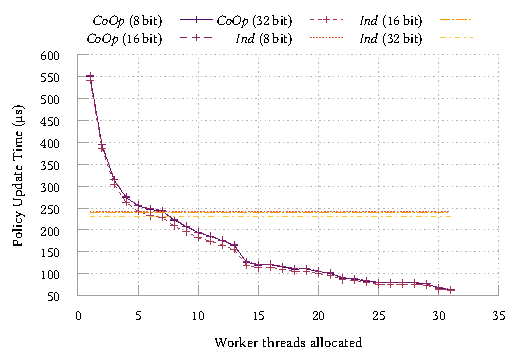
\includegraphics{plots/opal/rl-perf-tester/vary-core}
	}
	\caption{
		\Coopfw{}'s online learning performance improves with additional cores, on max size tasks (\num{129} work items). This requires \num{8} workers to offer greater online throughput than single-threaded in-NIC RL. Sharper performance increases occur when a new physical core is added (\numrange{7}{8}) or the scheduler works around a bottleneck (\numrange{13}{14}).\label{fig:vary-core}}
\end{figure}

\begin{figure}
	\resizebox{\resultplotwidth}{!}{
		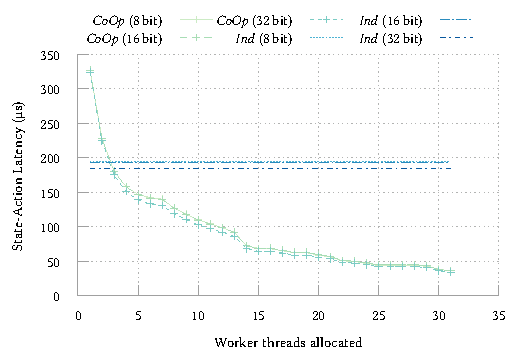
\includegraphics{plots/opal/rl-perf-tester/vary-core-latency}
	}
	\caption{\Coopfw{}'s action latencies similarly improve with more cores. This requires \num{3} workers (4 total contexts) to improve upon the state-action latency of single-threaded in-NIC RL.\label{fig:vary-core-latency}}
\end{figure}

\Cref{fig:vary-work,fig:vary-work-latency} show how policy complexity affects update cost and state-action latency respectively, scaling from a bias tile up to the full DDoS policy size.\footnote{Input vectors here all have 20 elements regardless of the policy design.}
\Coopfw{} always produces an action in less time than \Indfw{}, but requires at least one state-based tile to excel in online learning.
%We note that this is a trivial case, in that the use of \emph{only} a bias tile negates the need for any input state (similar to a multi-arm bandit problem).
We note that this is a trivial case, as using \emph{only} a bias tile returns a single preference list regardless of input state.

We found that a key aspect of in-NIC execution is that it allows far tighter bounds on tail latency compared to host offloading.
Examining the state-action latencies in \cref{tab:lats}, we see that \num{99.99}\nthscript{th} percentile latencies exceed the median by \qtylist{0.58;0.66}{\percent} for \Indfw{} and \Coopfw{}, respectively.
Similar results were observed for other bit depths.
By contrast, host-based tail latencies are at least \qty{40.53}{\percent} greater even when the parallel worker count is at or below the physical core count.
We show the cumulative distributions of these in detail (\cref{fig:lat-cumul}), noting how just one additional CPU-intensive task---potentially automated system updates, scans, or another vNF/traffic processing task---impacts tail latencies further (\emph{Float(Over)}).

\begin{figure}[t]
	\resizebox{\resultplotwidth}{!}{
		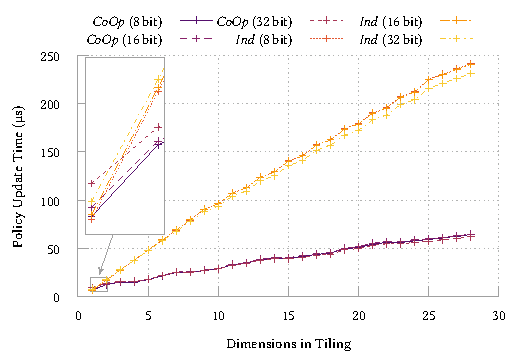
\includegraphics{plots/opal/rl-perf-tester/vary-work}
	}
	\caption{\Coopfw{} fully processes updates faster than \Indfw{}---thus has higher online performance---on almost all policy sizes. Lower bit depths are more effective on simpler policies.\label{fig:vary-work}}
\end{figure}

\begin{figure}
	\resizebox{\resultplotwidth}{!}{
		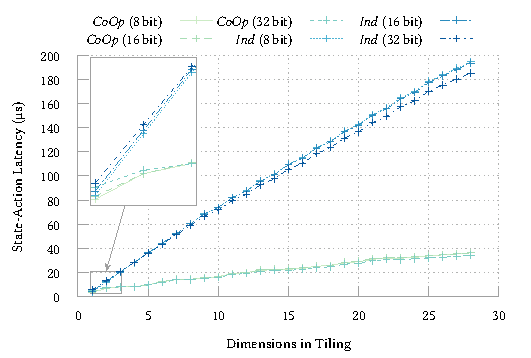
\includegraphics{plots/opal/rl-perf-tester/vary-work-latency}
	}
	\caption{State-action latency scales with additional work in a similar manner to overall processing time; though \qty{32}{\bit} firmwares become more effective sooner (at \num{3} work items).\label{fig:vary-work-latency}}
\end{figure}

\begin{figure}
	\centering
	\begin{subfigure}{\linewidth}
		\resizebox{1.0\linewidth}{!}{
			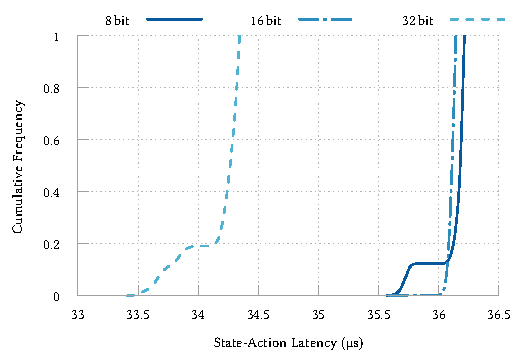
\includegraphics{plots/opal/rl-perf-tester/latency-cumul-thesis}
		}
		\caption{\approachshort's \Coopfw{} design achieves consistent, tight latency bounds.}
	\end{subfigure}

	\begin{subfigure}{\linewidth}
		\resizebox{1.0\linewidth}{!}{
			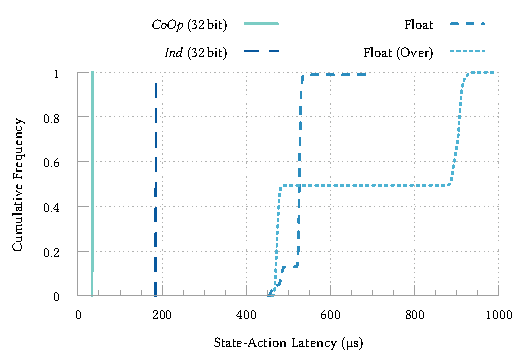
\includegraphics{plots/opal/rl-perf-tester/latency-cumul-broad-thesis}
		}
		\caption{Tail latencies suffer in hosts---particularly when oversubscribed.}
	\end{subfigure}
	\caption{Cumulative state-action latency plots for \approachshort{} and host-based execution.\label{fig:lat-cumul}}
\end{figure}

A noteworthy trend is that \qtylist{8;16}{\bit} versions of \approachshort{} consistently underperform compared to \qty{32}{\bit}, except for smaller workloads (seen in the zoomed portions of \cref{fig:vary-work,fig:vary-work-latency}).
This occurs even though our implementation is optimised to read and write policy data in batches (achieving fewer I/O operations).
We see this because the native register width on the NFP is \qty{32}{\bit}, and so the compiler must emit extra instructions around arithmetic operations to correctly load and update values.
This matches \qty{32}{\bit} becoming dominant in complex workloads: higher dimension tilings require more arithmetic operations.
Most of the I/O comes \emph{after} this step, causing ALU use to dominate.
This also explains why \qty{32}{\bit} becomes the best choice at different policy complexities for online (\cref{fig:vary-work}, 10 dims) and offline (\cref{fig:vary-work-latency}, 3 dims) agents, where hashtable accesses and a \texttt{memcpy} of the state vector fall into the serial portion of the online algorithm.
Smaller bit depths still give a \qtyrange{2}{4}{\times} saving in memory for policy storage (enabling more fine-grained or complex policies), in exchange for slightly worse latency and throughput.
To overcome this, we investigated bit-stuffing several values into a single word during atomic writeback (as the platform offers both \qtylist{32;64
}{\bit} atomic addition).
This is analogous to SIMD through clever use of padding bits, but we found that manipulating tiles into the correct format added \qty{10}{\percent} extra overhead.

\paragraph{Work allocation}
\Cref{fig:work-alloc-32} shows that our heuristic allocator (\emph{Balanced}) is key in achieving consistent sub-\qtylist{35;65}{\micro\second} latencies/update times, respectively.
The trend is repeated for all bit depths.
The constant difference between \emph{Action} and \emph{Update Prep} scales linearly with bit depth, matching storage and lookup work in the serial portion of \emph{ParSa} (plots omitted).
The severe underperformance of the \emph{Na\"{i}ve} allocator confirms that work item complexity is correlated with its index, as batching work in contiguous chunks gives some workers only high-dimensionality tilings.
The minor gap in lower bound performance between the \emph{Random} and \emph{Balanced} allocators suggests that further optimisations can be made.
We expect that closing or exceeding this gap may require more complex modelling of hardware thread interactions, which lies far beyond the scope of in-NIC scheduling.
Some additional complexity may be tolerated, subject to code store limits---scheduling runs exactly once per configuration change, so does not impact per-action code.

\begin{figure}
	\resizebox{\resultplotwidth}{!}{
		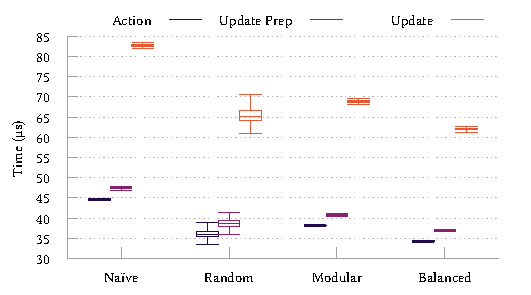
\includegraphics{plots/opal/rl-perf-tester/work-strat-32bit}
	}
	\caption{Action/update compute times in a \qty{32}{\bit} \Coopfw{} agent under different work schedulers.\label{fig:work-alloc-32}}
\end{figure}

\begin{figure}
	\resizebox{\resultplotwidth}{!}{
		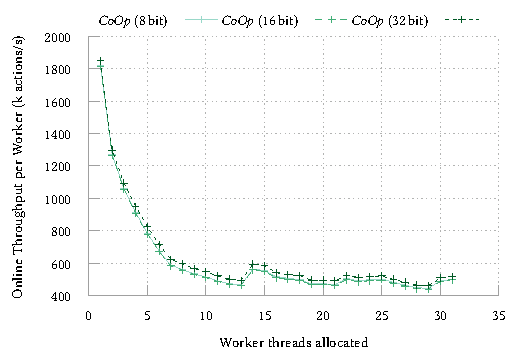
\includegraphics{plots/opal/rl-perf-tester/vary-core-tput-on-per}
	}
	\caption{Throughput per added worker in a \Coopfw{} agent.\label{fig:tput-per-core}}
\end{figure}

An interesting aspect of \Coopfw{} and \emph{ParSa} is that adding cores has both diminishing returns and key thresholds to pass.
Consider \cref{fig:tput-per-core}, where the throughput per worker decreases with cores but occasionally increases sharply.
Later downward ticks (\numrange{25}{29} workers) correspond to plateaus in throughput.
This is a problem stemming from the granularity of work items (i.e., tilings in \emph{ParSa}), where our scheduler cannot find a better solution to a bottleneck until extra cores are allocated.
We measured individual work items in state-action computation to take a mean \qtylist{5.2; 6.2; 9.7; 11.0}{\micro\second} for bias, CLS, CTM and IMEM tilings respectively.
Though we have a \qty{4.2}{\times} factor of task oversubscription, it is clear that latencies are eventually bound below by the length of the longest task.

\paragraph{End-to-end RL latency}
%?? PCIe RTT is 10us (neugebauer, BNN NFP paper), NFP RTT is 18us (own measurements). EMEM Ring one-way is 120ns.
%?? Cziva~\parencite[pp.113]{DBLP:phd/ethos/Cziva18} discusses vNF times.
%?? reference the inference times brought up in Taurus?
Referring to \cref{fig:state-slip}, we take $t_2$ from \cref{tab:lats} for host and in-NIC processing times, and substitute $t_1+t_3$ for the state packet round-trip time to the decision site:
\begin{description}
	\item[In-NIC.] As described in \cref{sec:agent-environment-communication}, EMEM rings have a median one way delay cross-island of \qty{140}{\nano\second}, giving a \emph{median \qty{34.63}{\micro\second} end-to-end inference latency}.
	\item[Dedicated Collector.] Offloads hosted in this manner will employ DPDK to maximise performance, giving one-way PCIe delays of \qtyrange{0.9}{2.3}{\micro\second} for network packets~\parencite{DBLP:conf/sigcomm/NeugebauerAZAL018}.
	A UDP packet carrying \num{20} elements of state in \approachshort{} is \qty{128}{\byte}, so costs \qty{1}{\micro\second} to forward, and the reply state-action pair is slightly larger.
	\emph{This gives an end-to-end inference latency of \qty{517.9}{\micro\second}}.
	\item[vNF Offload.] \Textcite{DBLP:journals/cm/CzivaP17} show that more lightweight vNF frameworks like GNF~\parencite{DBLP:journals/cm/CzivaP17} and ClickOS~\parencite{DBLP:conf/nsdi/MartinsAROHBH14} add \qtyrange{45}{55}{\micro\second} \emph{additional} RTT latency above PCIe costs.
	\emph{This gives an end-to-end inference latency of \qty{572.9}{\micro\second}}.
\end{description}
Using these estimates, in-NIC classical RL inference offers \qtylist{14.96;16.54}{\times} speedups in latency over collector and vNF deployments respectively (assuming no steering cost in either case).
We also contrast these against deep RL policies on network tasks, which can take \qty{3}{\milli\second} to compute~\parencite{DBLP:journals/corr/abs-1910-04054}---2 orders of magnitude above \approachshort{} with identically sized (20-dim) input vectors.
%In the name of fairness, we assume that rule installation uses same mechanism we recommend, but show how bad it can get? I.e. with rule installation costs etc.

\paragraph{Co-existence with the dataplane}
Our setup met \qty{40}{\giga\bit\per\second} for packet sizes $\ge$\qty{256}{\byte}.
%For frame sizes of \qtylist{64;128;256}{\byte} input traffic rates were \qtylist{17.4;32.9;37.0}{\giga\bit\per\second} respectively (\qtylist[per-symbol=p,sticky-per=true]{33.9;32.2;18.1}{\mega\packet\per\second}).
For frame sizes of \qtylist{64;128}{\byte}, input traffic rates were \qtylist{17.4;32.9}{\giga\bit\per\second} respectively (\qtylist[per-symbol=p,sticky-per=true]{33.9;32.2}{\mega\packet\per\second}).
Passing this traffic over the NFP device running \approachshort, no packet losses were incurred at any rate of RL actions.

We show the effect of RL workloads on the round-trip latencies of cross traffic through \cref{fig:dataplane-coop}.
As observed latencies do not obey a normal distribution (particularly \qtylist{256;1518}{\byte}, which are bimodal), we employ a one-tailed \emph{Mann-Whitney U test} to mark statistically significant population increases in latency ($p < 0.05$) with a ``+''.
In general, statistically significant latency increases concentrate around smaller packet sizes.
All (bar one) of these affected \nth{99} percentile latencies by under \qty{0.38}{\percent} (at most \qty{78}{\nano\second}).
This slight degradation can be explained by increased pressure on the NFP's \emph{Command Push-Pull} (CPP) bus, which is responsible for handling cross-island accesses to memory (particularly IMEM/EMEM) and other resources.
\approachshort{} places load on the CPP bus through its \inring{}/\outring{} EMEM rings and last-tier policy accesses.
This also explains the sensitivity of \qty{256}{\byte} packets to \approachshort{}---the NFP P4 toolchain segments packets, storing metadata (e.g., MAC prepend) and the first bytes of a packet in a \qty{256}{\byte} CTM block and parking their payloads in EMEM.
\qty{256}{\byte} packets overshoot this due to metadata, causing small I/O accesses at a high rate for packets sized around this cutoff.
%Regardless, this effect is small when observed.

The anomalous result is \qty{128}{\byte} packets at \num{3000} RL action/update computations per second, causing a \qty{222}{\nano\second} (\qty{1.18}{\percent}) increase, shown in \cref{fig:dataplane-example}.
This is observed through a shift of some packet latencies from the mode towards the tail, but no other changes in the distribution.
In the above context, we believe that the inbound request rate is weakly synchronised with inbound packets, causing a higher level of burstiness around accesses to the CPP bus.
We expect that dedicated hardware/FPGA designs can avoid this problem by having dedicated \inring{}/\outring{} access mechanisms for an \approachshort{} agent.

\begin{figure}
	\centering
	\begin{subfigure}{0.45\linewidth}
		\resizebox{1.0\linewidth}{!}{
%			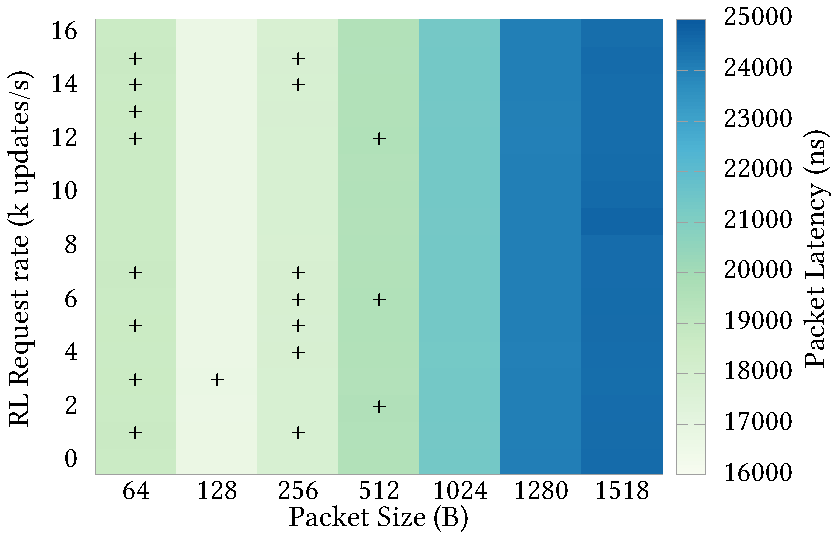
\includegraphics{../plots/build/stress/heat-latency-median}
			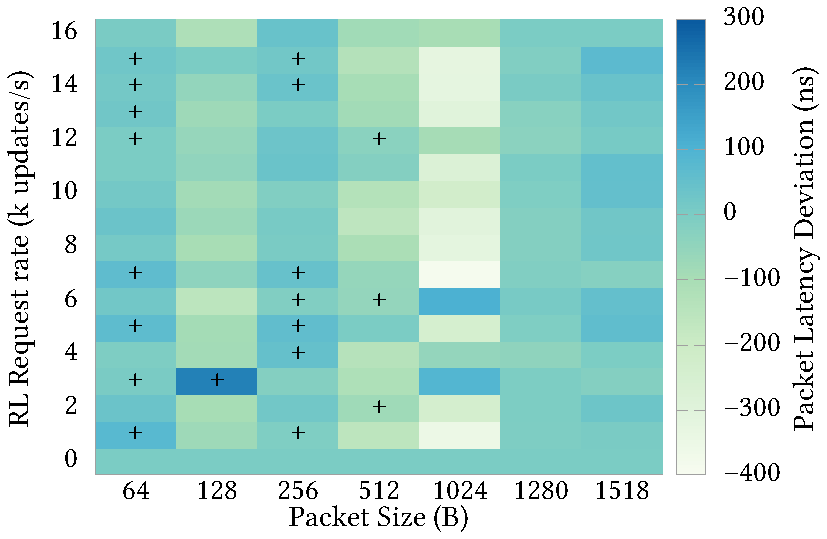
\includegraphics{plots/opal/stress/heat-latency-two-9-rel}
%			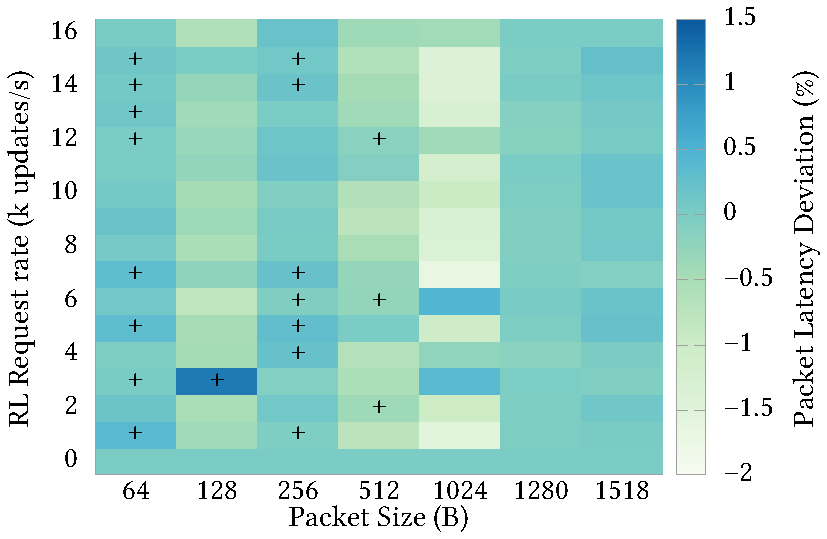
\includegraphics{../plots/build/stress/heat-latency-two-9-perc}
		}
		\caption{Deviations in \nth{99} percentile cross-traffic RTTs.\label{fig:dataplane-heat}}
	\end{subfigure}
	\hspace{0.05\linewidth}
		\begin{subfigure}{0.45\linewidth}
		\resizebox{1.0\linewidth}{!}{
			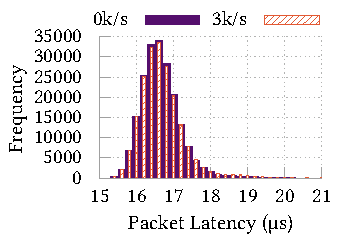
\includegraphics{plots/opal/stress/histo-128B-0-3-trim}
		}
		\caption{Distribution of RTTs for \qty{128}{\byte} packets for \numlist{0;3000} RL actions/s.\label{fig:dataplane-example}}
	\end{subfigure}
	\caption{Effects on tail latency of cross-traffic caused by different loads of off-path RL compute. Statistically significant increases in population latency are concentrated on smaller packet sizes, and are typically sub-\qty{78}{\nano\second}.\label{fig:dataplane-coop}}
\end{figure}

\paragraph{Resource requirements}
\Cref{tab:resources} shows how \approachshort{} consumes shared memory as it scales to fit a device's compute resources, compared with a simple P4 forwarding application.
As one program is installed per ME, these results represent the minimum and maximum resource use on a single island (i.e., without replacing P4 workers).
We observe negligible costs on shared EMEM ($\sim$\qty{4}{\mebi\byte}), incurred due to hashtables for past state and rewards.
The most significant costs arise due to policy data (\qty{405}{\kibi\byte} shared IMEM, \qty{90}{\kibi\byte} local CTM, \qty{15}{\kibi\byte} local CLS), which can be halved or quartered using \qtylist{16;8}{\bit} quantisation and remain constant regardless of compute unit usage.
This is a high upfront cost on per-island resources (CLS/CTM)---\approachshort{} leaves resources for other off-path dataplane applications, but is fairest from 3 cores onwards.

%Thread local storage in CLS for compute/register spilling scales with the number of MEs required (requiring \qtylist{13.77;15.49}{\percent} per-ME for \Indfw{}/\Coopfw) due to precaching and the space needed to hold tile lists.
%Due to the initial policy cost this falls below the fair share at 3 MEs, but always allows for co-existence with other asynchronous dataplane programs.

\begin{table}
\caption{NFP memory use due to \approachshort{} using \numlist{1;4} MEs (\qty{32}{\bit}). CLS and CTM are shared between all programs on the same island (placing our RL agent on i5), while EMEM and IMEM are shared between all NFP programs on a NIC.\label{tab:resources}}
\resizebox{\linewidth}{!}{
\begin{tabular}{
		@{}c
		S[table-format=4.2] S[table-format=2.2]
		S[table-format=4.2] S[table-format=2.2]
		S[table-format=4.2] S[table-format=2.2]
		S[table-format=2.2] S[table-format=2.2]
		S[table-format=3.2] S[table-format=2.2]
		@{}
	}
	\toprule Firmware & \multicolumn{2}{c}{EMEM} & \multicolumn{2}{c}{EMEM Cache} & \multicolumn{2}{c}{IMEM} & \multicolumn{2}{c}{i5.CLS} & \multicolumn{2}{c}{i5.CTM}\\
	& \multicolumn{1}{c}{\si{\mebi\byte}} & \multicolumn{1}{c}{\si{\percent}} & \multicolumn{1}{c}{\si{\kibi\byte}} & \multicolumn{1}{c}{\si{\percent}} & \multicolumn{1}{c}{\si{\kibi\byte}} & \multicolumn{1}{c}{\si{\percent}} & \multicolumn{1}{c}{\si{\kibi\byte}} & \multicolumn{1}{c}{\si{\percent}} & \multicolumn{1}{c}{\si{\kibi\byte}} & \multicolumn{1}{c}{\si{\percent}} \\
	\midrule Base P4 & 6776.67 & 88.24 & 268.52 & 2.91 & 858.28 & 10.48 & 0.00 & 0.00 & 0.00 & 0.00 \\
	\Indfw(1) & 6780.21 & 88.28 & 2541.08 & 27.57 & 1263.28 & 15.42 & 24.75 & 38.67 & 94.25 & 36.82 \\
	\Indfw(4) & 6780.22 & 88.28 & 2545.33 & 27.62 & 1263.28 & 15.42 & 51.18 & 79.97 & 107.00 & 41.80 \\
	\Coopfw(1) & 6779.12 & 88.27 & 1773.59 & 19.24 & 1263.28 & 15.42 & 22.41 & 35.01 & 90.00 & 35.16 \\
	\Coopfw(4) & 6779.12 & 88.27 & 1769.84 & 19.20 & 1263.28 & 15.42 & 52.16 & 81.49 & 90.00 & 35.16 \\
	\bottomrule
\end{tabular}
}
\end{table}

%\paragraph{The impact of bit depth}
%?? \Cref{fig:quant-acc}
%?? \qty{5}{\bit} mantissa suffices for $\ge$ \qty{90}{\percent} relative accuracy, so \qty{8}{\bit} is fine (1S + 2E + 5M), \qty{16}{\bit} is better.
%
%\begin{figure}
%	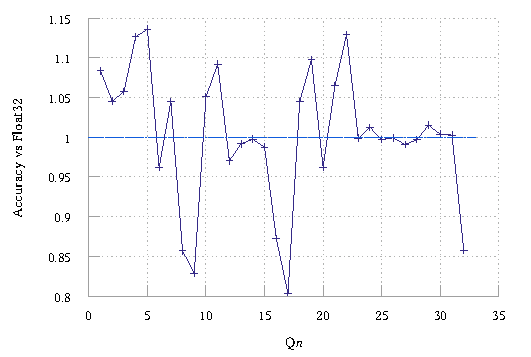
\includegraphics{../plots/build/marl-quant/accuracy-binary}
%	\caption{Normalised accuracy of a converted, pre-trained floating-point tile-coded policy after conversion to $32Qn$ fixed-point.}\label{fig:quant-acc}
%\end{figure}

\paragraph{Deployability}
Setup of \approachshort{} uses two packet types: \emph{setup}, which contains learning (hyper-)parameters and most aspects of a policy, and \emph{tiling}, which provides a list of state indices for tiling sets.
We found that setup and tiling packets take a mean \qtylist{27.03;16.69}{\micro\second} to be processed on \Indfw{}, allowing an agent to be swapped between online and offline operation (or repurposed for another task) painlessly.
Online/offline swaps are useful when an agent should cease learning (i.e., when performance has converged), or if a change in the environment suggests that more training is needed.
Tiling packet processing scales linearly with the number of \emph{tiling sets}, due to the needed precaching of tile set boundaries.
Online-offline swaps for \Coopfw{} exhibit similar cost, however the need for explicit scheduling means that policy/tiling \emph{structure} changes (including the first complete setup) take \qty{422.63}{\micro\second} for the full-size policy described above.
The time taken for \Coopfw{} to schedule its tasks was found to scale with the number of workers ($m$) and work items ($n$) as described earlier (\cref{sec:work-allocation}, $\mathcal{O}{\left(n\log{m}\right)}$).
Ignoring the trivial solutions, reducing the worker count to \num{1} costs a mean \qty{238.22}{\micro\second}, while placing a single task incurs \qty{53.79}{\micro\second}.
Policy \emph{data} changes require no additional work in any case, resolving purely to \texttt{memcpy}s.

We observed that firmware installation (i.e., changing from \Indfw{} to \Coopfw{}, bit depth, or increasing maximum policy sizes) took a mean time of \qty{38.83}{\second}.
In the event that appropriate firmwares are not pre-compiled, we found that compiling and linking both \approachshort{} and the P4 toolchain took around \qty{35}{\second}, while changing only \approachshort{} parameters required around \qty{25}{\second}.
These results show that \approachshort{} can be easily adapted and altered by network administrators once in place, and illustrates an advantage of SoC-based SmartNICs.
